% !TeX root = ./../memoria.tex
\chapter{Introducción específica}

\label{Capitulo2}

En este capítulo se desglosan las diferentes herramientas tanto de hardware como de software elegidas para el desarrollo del robot propuesto.

\section{Robot Operating System}

Comúnmente denominado ROS, es un framework de robótica de código abierto que fue diseñado originalmente para robots de uso académico. Sin embargo, al día de hoy su uso se ha extendido tanto a la industria como al público aficionado.

ROS ofrece un variado \textit{set} de herramientas que facilitan las tareas del roboticista en funciones como envío y recepción de mensajes, computación distribuida e implementación de algoritmos para aplicaciones robóticas.

\subsection{Organización de archivos}\label{sec:organizacionArchivos}

Es adecuado considerar a ROS como algo más que un framework de desarrollo y referirnos a el como un ``meta sistema operativo'', ya que ofrece no solo herramientas y bibliotecas sino también funciones similares a las de un sistema operativo. Entre ellas, podemos citar su abstracción del hardware, el manejo de paquetes, además de un completo \textit{toolchain} de compilación. Así también, tal como en un sistema operativo ``real'', los archivos que componen ROS se encuentran organizados en el disco duro de una manera particular, como se indica en la figura \ref{fig:rosSistemaDeArchivos}.

\begin{figure}[ht]
    \centering
    \def\svgwidth{350pt}
    \input{./Figures/estructura_archivos_ros.pdf_tex}
    \caption{Organización de archivos en ROS}
    \label{fig:rosSistemaDeArchivos}
\end{figure}

\newpage
A continuación se detalla en qué consiste cada uno de los bloques que componen la organización de archivos:
\begin{itemize}
    \item \textbf{Paquetes}: los paquetes de ROS representan la unidad básica de software en la plataforma. Contienen uno o más programas de ROS (nodos), bibliotecas, archivos de configuración, etc, que son organizados como una unidad coherente.
    \item \textbf{Manifiesto del paquete}: está representado por un archivo único dentro del paquete que contiene información sobre este tales como el nombre, autor, tipo de licencia, dependencias, banderas de compilación, etc. El archivo \file{package.xml} encontrado en la raíz del paquete es su propio manifiesto.
    \item \textbf{Metapaquete}: hace referencia a uno o más paquetes usualmente relacionados entre sí, pero sin estar necesariamente acoplados fuertemente unos con otros. El software provisto con este proyecto es un metapaquete.
    \item \textbf{Manifiesto del metapaquete}: similar al manifiesto del paquete, con la diferencia que este puede incluir dependencias a de tiempo de ejecución hacia otros paquetes.
    \item \textbf{Mensajes}: representados con la extensión \file{.msg}, son los tipos de datos utilizados por ROS internamente para comunicar los distintos procesos entre sí. El usuario puede definir tipos de mensajes personalizados con campos adaptados a sus necesidades en del directorio \file{msg} dentro del paquete.
    \item  \textbf{Servicios}: representados con la extensión \file{.srv}, representan interacciones del tipo solicitud/respuesta entre distintos procesos. Los formatos tanto para solicitud como para respuesta pueden definirse en el directorio \file{srv} dentro del paquete.
    \item \textbf{Repositorios}: la gran mayoría de los paquetes de ROS son mantenidos utilizando un sistema de control de versiones (SCV) tales como Git, Mercurial o SVN. Es común encontrar metapaquetes definidos dentro de un mismo único repositorio. Este es el caso para el repositorio provisto en este trabajo.
\end{itemize}

\subsection{Arquitectura interna}
ROS está construido sobre una arquitectura basada en grafos, esto significa que las tareas de cómputo son realizadas a través de una red de procesos llamados nodos. Esta red es denominada \textit{Computation Graph} o grafo de cómputo.

Los principales componentes de este grafo son los nodos, el \textit{master} o maestro, el \textit{parameter server} o servidor de parámetros, además de los mensajes, tópicos, servicios y \textit{bags} o bolsas. Cada uno de estos elementos contribuye al funcionamiento del \textit{Computation Graph} con una funcionalidad específica. Los elementos que lo componen, mostrados en la figura \ref{fig:computationGraph}, se describen a continuación:

\newpage

\begin{figure}[ht]
    \centering
    \def\svgwidth{350pt}
    \input{./Figures/ros_computation_graph.pdf_tex}
    \caption{Estructura del \textit{Computation Graph} de ROS.}
    \label{fig:computationGraph}
\end{figure}

\begin{itemize}
    \item \textbf{Nodos}: son los procesos que realizan las tareas de cómputo dentro del robot, que pueden comunicarse unos con otros a través de la API de ROS. Esto resulta particularmente útil cuando distintos nodos necesitan compartir información entre sí. En ROS se fomenta el uso de múltiples nodos que realicen procesos sencillos por sobre procesos grandes y complejos que abarquen toda la funcionalidad.
    \item \textbf{Master}: el ROS Master se encarga de buscar y registrar los diferentes componentes que interactúan en el sistema. Esto posibilita que diferentes nodos sean capaces de ``encontrarse'' mutuamente, intercambiar mensajes o invocar servicios. En un sistema distribuido, el master debe ejecutarse solamente en una de las computadoras.
    \item \textbf{Servidor de parámetros}: el servidor de parámetros o \textit{parameter server}, permite mantener la información utilizada en configuración de los nodos almacenada en una ubicación central. Esto permite a cada uno de los nodos a acceder y modificar dichos valores.
    \item \textbf{Mensajes}: los nodos se comunican entre sí mediante mensajes, estructuras de datos cuyos campos pueden editarse y permiten ser enviados entre sí. Existen tipos de mensajes estándares (enteros, flotantes, booleanos, etc.) así como también es posible definir mensajes propios, adaptados a las necesidades de la aplicación.
    \item \textbf{Tópicos}: cada mensaje en ROS es transportado utilizando buses llamados tópicos. Cuando un nodo envía un mensaje a través de un tópico, se puede decir que el nodo está ``publicando un tópico''. Asimismo cuando un nodo recibe un mensaje a través de un tópico, se puede decir que el nodo está ``subscripto al tópico''. El nodo publicante y el suscriptor no tienen información sobre su mutua existencia, por lo que es posible que existan nodos que publiquen en tópicos sin suscriptores o viceversa, es decir nodos suscriptos a tópicos sin publicantes.
    \item \textbf{Servicios}: en determinadas aplicaciones, el mecanismo de publicador/suscriptor definido en el ítem anterior podría no ser adecuado. Por ejemplo, en ciertos casos es necesaria una interacción del tipo solicitud/respuesta. En dichas situaciones un nodo podría solicitar la ejecución de un procedimiento rápido por parte de otro nodo y el envío de una respuesta con el resultado de dicho cálculo.
    \item \textbf{Logging}: ROS provee un sistema de registro o \textit{logging} denominado rosbag (bolsa), que se utiliza para almacenar información publicada en los tópicos activos, como por ejemplo la proveniente de un sensor que podría ser difícil de generar una y otra vez, pero que a su vez resulta necesaria para depurar determinados algoritmos. Un rosbag permitiría en este caso generar la información una única vez para luego reproducirla como si fuese una grabación las veces que resulte necesario.
\end{itemize}

\subsection{Herramienta RViz}

La herramienta RViz (o ROS Visualization tool) es la herramienta oficial de visualización ROS, que permite representar de manera gráfica la información transmitida a través de los distintos tópicos. Posee soporte nativo para la mayoría de los mensajes estándar y permite además, expandir su funcionamiento mediante \textit{plugins} que posiblitan entre otras cosas, visualizar mensajes definidos por el usuario. La configuración estándar de RViz permite visualizar la configuración de articulaciones (o \textit{joints}) y enlaces (o \textit{links}) de un robot como se muestra en la figura \ref{fig:rviz}.

\begin{figure}[ht]
    \centering
    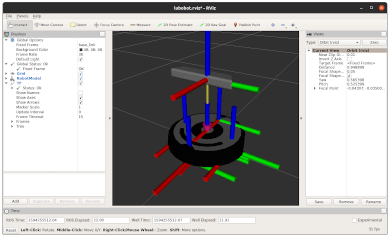
\includegraphics{./Figures/rviz.png}
    \caption{Interfaz gráfica de RViz donde se muestran los \textit{links} y \textit{joints} del robot Lubobot.}
    \label{fig:rviz}
\end{figure}


\subsection{Formato universal de descripción de robots URDF}

El formato universal de descripción de robots o \textit{Universal Robot Description System}, comúnmente referido como URDF es un formato estándar para representación de modelos conformados por múltiples piezas conectadas entre sí, como es el caso de brazos robóticos o líneas de ensamblaje. Este es ampliamente utilizado dentro del ecosistema de ROS, plataforma donde vio su origen aunque al día de hoy su uso se ha extendido a herramientas externas como MATLAB, que permite importar archivos URDF directamente a su \textit{toolbox} de robótica.

\subsection{Biblioteca rosserial}\label{sec:rosserial}

Es un protocolo para la transmisión serial de mensajes y multiplexación de múltiples tópicos y servicios de ROS sobre un \textit{character device} tal como un puerto UART o un \textit{socket} de red.
Además de la definición del protocolo de serialización en si mismo, rosserial se compone de otros dos elementos principales:
\begin{itemize}
    \item \textbf{bibliotecas cliente}: permiten la integración de nodos ROS en diferentes plataformas, apuntando principalmente a sistemas embebidos. Dichas librerias son especializaciones de una clase base, escrita en ANSI C++ para mayor compatiblidad y denominada rosserial\_client. Para este trabajo se realizó un \textit{port} de dicha biblioteca a la plataforma STM32CubeHAL.
    \item \textbf{Interfaz con ROS}: las bibliotecas cliente requieren de que haya un nodo corriendo en la computadora \textit{host} que funcione como puente entre el serie y la red de ROS, que se encarga de des-serializar y serializar los mensajes que llegan y se despachan, respectivamente. La participación de los distintos actores involucrados en el uso de rosserial se muestran en la figura \ref{fig:rosserial}.
\end{itemize}

\begin{figure}[ht]
    \centering
    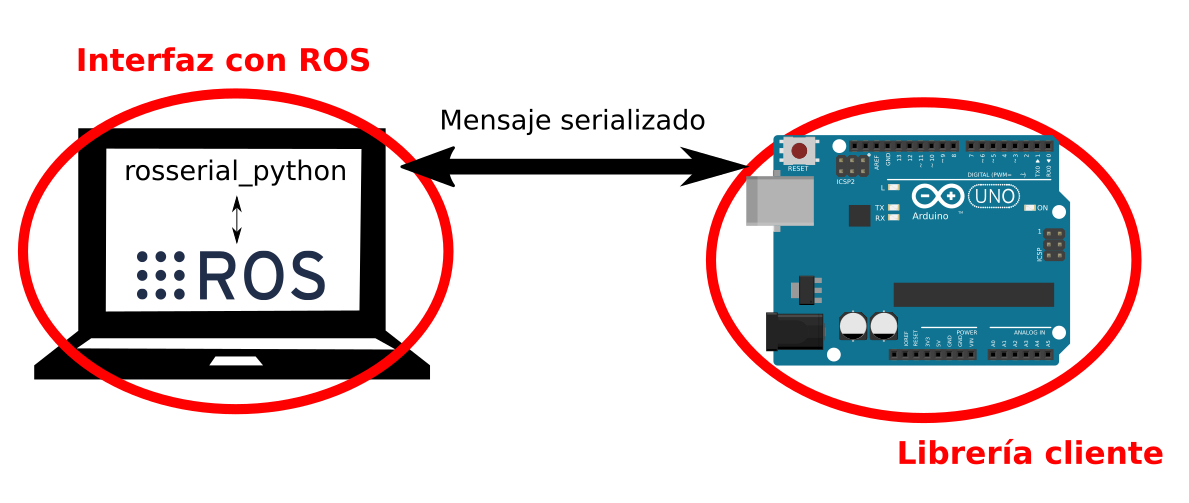
\includegraphics[scale=0.6]{./Figures/rosserial.png}
    \caption{Interacción entre ROS y rosserial que se ejecutan en un microcontrolador.}
    \label{fig:rosserial}
\end{figure}

\subsection{Transformación de coordenadas con TF}

Dentro del campo de la robótica resulta indispensable trabajar con múltiples sistemas de referencia tanto dentro del mismo robot (a la hora de representar el estado de sus articulaciones) así como para representar su estado en su universo de acción o mundo, como puede ser un mapa. Con la finalidad de y simplificar este tipo de cálculos ROS incorpora el paquete llamado TF.

Esta biblioteca fue diseñada para proveer una manera estándar para mantener el registro de los \textit{coordinate frames} o marcos de coordenadas y de realizar las transformaciones entre si mismas en todo el robot, de modo a que los usuarios puedan consumir la información de manera ordenada y sin la necesidad de ocuparse de generar las transformaciones en forma manual \citep{PAPER:3}.

TF puede operar de forma transparente en sistemas distribuidos, muy típicos en el entorno ROS. Esto significa que toda la información sobre los marcos de coordenadas de un robot se encuentran disponibles para todos los componentes de un sistema ROS en cualquiera de las computadoras que componen el sistema.

En la figura \ref{fig:tf} se visualiza un robot con múltiples articulaciones. Dado que la pose de estas se encuentra sujeta a cambios en el tiempo, también así lo hacen sus transformaciones. Por este motivo TF se encarga de monitorearlas en todo momento, lo que provee al robot la capacidad de responderse preguntas como las siguientes:

\begin{itemize}
    \item ¿a dónde se encontraba el \textit{frame} ``cabeza'' con respecto al \textit{frame} ``mundo'' hace cinco segundos?
    \item ¿cuál es la pose del objeto sostenido en mi \textit{gripper} con respecto a mi base?
    \item ¿cuál es la pose actual del \textit{frame} ``base'' en el \textit{frame} ``mapa''?
\end{itemize}


\begin{figure}[ht]
    \centering
    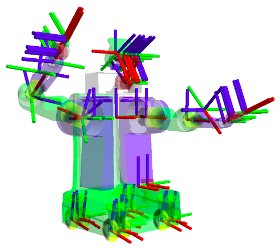
\includegraphics[scale=0.8]{./Figures/tf.png}
    \caption{Ejemplo de los \textit{frames} registrados con TF en el robot PR2, de la compañía Willow Garage.\protect\footnotemark}
    \label{fig:tf}
\end{figure}

\footnotetext{Imagen tomada de \url{http://wiki.ros.org/tf?action=AttachFile&do=get&target=frames2.png}}

\subsection{Paquete de localización robot\_localization}\label{sec:robotLocalization}

El paquete robot\_localization es una colección de estimadores no lineales para robots en espacios 2D y 3D, aunque para el aclance de este trabajo solo se hace hincapié en entornos en dos dimensiones.

Cada uno de estos estimadores permite fusionar un número arbitrario de sensores (IMUs, fuentes de odometría, sistemas de localización interna, receptores GPS, etc.) a su salida genera un vector de 15 dimensiones con el estado del robot ($x$, $y$, $z$, $roll$, $pitch$, $yaw$, $\dot{x}$, $\dot{y}$, $\dot{z}$, $\dot{roll}$, $\dot{pitch}$, $\dot{yaw}$, $\ddot{x}$, $\ddot{y}$, $\ddot{z}$).

Todos los estimadores de estados controlados por este paquete aceptan mediciones provenientes de cualquier sensor de pose siempre y cuando los mismos publiquen en alguno de los tres tipos de mensaje compatibles que se citan a continuación:

\begin{itemize}
    \item \textbf{nav\_msgs/Odometry}: posición y orientación, y velocidades lineal y angular.
    \item \textbf{sensor\_msgs/Imu}: orientación, velocidad angular y aceleración lineal.
    \item \textbf{geometry\_msgs/PoseWithCovarianceStamped}: posición y orientación.
    \item \textbf{geometry\_msgs/TwistWithCovarianceStamped}: velocidad lineal y angular.
\end{itemize}

Para este trabajo se hace uso de los dos primeros tipos de mensajes citados en la lista.

En base a estas mediciones, los estimadores publican los valores de estado filtrados de posición, orientación y velocidades lineal y angular mediante un mensaje del tipo \file{nav\_msgs/Odometry} y opcionalmente, valores de aceleración (no utilizadas en el presente trabajo).

El sotware permite a los usuarios decidir cuál de los campos de información proveidos por los sensores van a ser tomados en cuenta para la fusión en el estimador. Por este motivo, como parte de la configuración del paquete es necesario definir una matriz de booleanos para cada una de las fuentes de información o sensores para informar al estimador cuáles son los campos a tener en cuenta. A continuación se muestra la matrix completa de variables requerida para la configuración de cada una de las fuentes:

\[
    \begin{bmatrix}
        x          & y           & z         \\
        roll       & pitch       & yaw       \\
        \dot{x}    & \dot{y}     & \dot{z}   \\
        \dot{roll} & \dot{pitch} & \dot{yaw} \\
        \ddot{x}   & \ddot{y}    & \ddot{z}
    \end{bmatrix}
\]


\subsection{Paquete de navegación ros\_navigation\_stack}\label{sec:rosNavigation}

El paquete de navegación de ROS, usualmente referido como \textit{navigation stack}, es un set de algoritmos que hace uso de los sensores y las fuentes de odometría disponibles para controlar al robot es decir, le permiten moverse de un punto conocido a otro del mapa a la vez que mantiene una estimación de su posición en el espacio a cada instante.

Para que un robot pueda hacer uso de este paquete correctamente, es necesario que se satisfaga una serie de requisitos:
\begin{itemize}
    \item Solo puede utilizarse en robots con ruedas en configuración de tracción diferencial u holonómica. Cabe mencionar que el robot presentado en este trabajo es de configuración diferencial.
    \item Es necesario que el robot publique la información sobre las relaciones entre las posiciones de todas las articulaciones y sensores que lo componen.
    \item El robot deberá reportar sus velocidades lineal y angular utilizando un mensaje estándar de ROS.
    \item Un sensor del tipo LIDaR 2D deberá estar presente en el robot para generar el mapa y para el proceso de localización. Alternativamente, es posible utilizar otros tipos de sensores como cámaras de profundidad o \textit{depth cameras} o SONAR, siempre y cuando la información recolectada se publique con el tipo de mensaje adecuado.
\end{itemize}

En la figura \ref{fig:navigationStack} se puede apreciar cómo se encuentra organizado el paquete de navegación, el que utiliza dos mapas de obstáculos, uno local y otro global, que son construidos a partir de la información generada por el escáner láser en conjunto con el sistema de navegación. El mapa global es más extenso en dimiensiones que el local y está diseñado para el cálculo de trayectorias globales. Por otro lado, el mapa local es usualmente más acotado pero con mayor detalle y su objetivo es el de evadir obstáculos cercanos.

\begin{figure}[ht]
    \centering
    \def\svgwidth{350pt}
    \input{./Figures/navigation_stack.pdf_tex}
    \caption{Configuración típica del paquete de navegación en ROS.}
    \label{fig:navigationStack}
\end{figure}

Los mapas global y local son utilizados por los planeadores global y local, respectivamente. El planeador global se encarga de generar un plan para ir de un punto a otro del mapa homónimo. Por otro lado, el local se encarga de controlar los distintos actuadores del robot, por ejemplo las ruedas, para llevar a cabo el plan global pero a la vez que esquiva los obstáculos cercanos que puedan aparecer, incluso si los mismos no se encontrasen registrados en el mapa global. Esto resulta especialmente útil a la hora de esquivar obstáculos nuevos, hasta el momento desconocidos.

\section{Conceptos de robótica móvil}

En esta sección se introduce a algunos conceptos de robótica móvil que resultan de especial importancia para la comprensión en detalle del trabajo expuesto en los siguientes capítulos.

\subsection{Cinemática de un robot de tracción diferencial}

Este tipo de tracción se caracteriza por disponer de dos ruedas situadas sobre el mismo eje horizontal con la particularidad de poder ser comandadas individualmente, es decir, el sentido y velocidad de giro de cada una es independiente de la otra.

Las ventajas de este tipo de movimiento que lo hacen especialmente útil para aplicaciones como las del presente trabajo son las siguientes:

\begin{itemize}
    \item Los cálculos matemáticos requeridos para describirlo son sencillos de calcular y en consecuencia, de aplicar.
    \item Hace posible realizar giros de 360 grados alrededor del eje vertical.
    \item Es la opción elegida por los fabricantes para bases móviles comerciales de bajo costo, como el Roomba 500 descripto en la sección \ref{sec:roomba}.
\end{itemize}

\begin{figure}[ht]
    \centering
    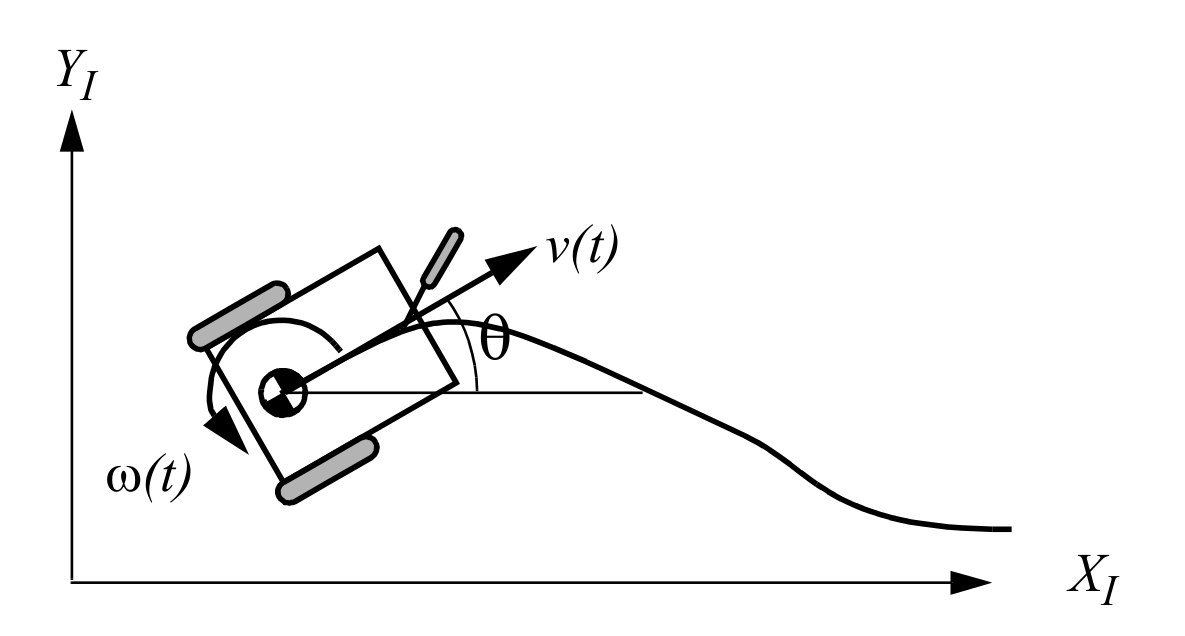
\includegraphics[scale=0.8]{./Figures/diff_drive.png}
    \caption{Descripción de la trayectoria de un robot de tracción diferencial con rueda ``loca'' o \textit{caster}.}
    \label{fig:diffdrive}
\end{figure}

Como se muestra en la figura \ref{fig:diffdrive}, es posible controlar la trayectoria descripta por el robot en un plano $(X,Y)$ mediante la manipulación de las velocidad lineal $v$ y angular $w$ del conjunto \citep{BOOK:3}. En un sistema de tracción diferencial, las fórmulas que describen la velocidad lineal $v$ y angular $w$ se muestran en la ecuacion \ref{eq:diffDriveLinear} y \ref{eq:diffDriveAngular}, respectivamente.

\begin{equation}
    \label{eq:diffDriveLinear}
    v = \frac{1}{2} \frac{V_i + V_d}{V_i - V_d}
\end{equation}

\begin{equation}
    \label{eq:diffDriveAngular}
    w = \frac{V_i - V_d}{l}
\end{equation}

donde $V_i$ y $V_d$ representan las velocidades de desplazamiento lineal de las ruedas izquierda y derecha, respectivamente y $l$ es la distancia entre ambas ruedas sobre el eje de giro.

Se generan tres casos particulares dignos de mención:
\begin{itemize}
    \item Si $V_i = V_d$, se tendrá un movimiento lineal en línea recta por lo que la velocidad angular $w$ será nula.
    \item Si $V_i = - V_d$, entonces solo habrá velocidad angular $w$ y la velocidad lineal $v$ del conjunto será nula.
    \item Si $V_i = 0$, entonces se tendrá una rotación en sentido anti-horario alrededor de la rueda izquierda con un radio de giro $l$. Se verá el mismo efecto para $V_d = 0$, esta vez con rotación en sentido horario.
\end{itemize}

\subsection{Odometría basada en encoders}

La odometría es el estudio de la estimación de la posición de robots con ruedas durante la navegación, para la que se utiliza información sobre la rotación de las ruedas que permiten estimar cambios en la posición de la base móvil en el tiempo, como se muestra en la figura \ref{fig:navigation}.

Este modelo supone que el desplazamiento de las ruedas es traducible al desplazamiento real del robot. Sin embargo, en la práctica esto no es necesariamente cierto debido a la presencia de distintos tipos de errores tales como ruedas desiguales, medidas inexactas o el resbalamiento de las ruedas en la superficie \citep{PAPER:2}. Estos motivos son los causantes de un error acumulativo no acotado que hacen que este método solo resulte apto para estimaciones en intérvalos de distancia pequeños.

Resulta necesario enriquecer esta estimación mediante su fusión con otras fuentes de información diferentes, tales como las que proveen las unidades de medición inercial, odometría visual mediante cámaras, sensores de profundidad, etc a modo de obtener una estimación final mas precisa. En este trabajo se aborda el proceso de fusión de varios de los sensores mencionados, y permite además, agregar otras fuentes de información con relativa facilidad.

\begin{figure}[ht]
    \centering
    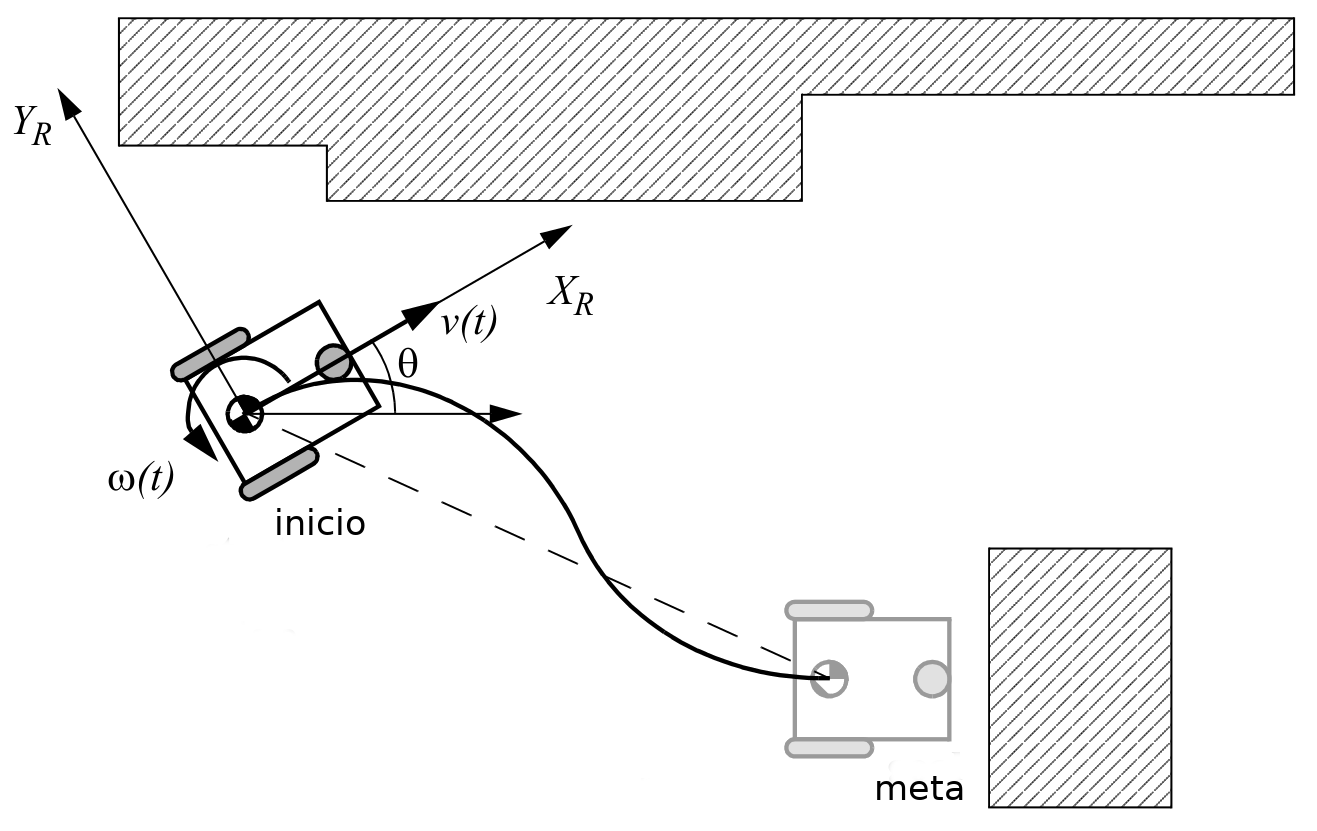
\includegraphics[scale=0.8]{./Figures/navigation.png}
    \caption{Trayectoria real descripta por un robot de tracción diferencial.}
    \label{fig:navigation}
\end{figure}

\section{iRobot Roomba 500}\label{sec:roomba}

El Roomba es un robot de limpieza fabricado y comercializado por la compañía iRobot. El primer modelo salió al mercado en el año 2002 y ha recibido siete actualizaciones desde entonces. En cada iteración, se han mejorado aspectos tanto de diseño como funcionalidad y esto le ha permitido mantenerse como el robot de limpieza con más unidades vendidas en el mundo.

Todos los Roomba incluyen una serie de sensores táctiles, ópticos y acústicos que le permiten detectar obstáculos, residuos, así como escalones o desniveles en el piso.

A nivel de locomoción, se catalogan como robots móviles con ruedas y utilizan el tipo de tracción diferencial, que consiste en dos ruedas motrices independientes que le permiten ejecutar giros de 360 grados. Esto es posible sin que el robot deba incurrir en desplazamiento lineal alguno como en el caso de los automóviles, por ejemplo.

La base móvil utilizada para este trabajo consiste en un Roomba de la serie 500 como el mostrado en la figura \ref{fig:roomba}, que fue introducido al mercado en el año 2007 y se comercializó hasta el 2017. Actualmente es posible conseguir estos equipos en condicion de usado o remanufacturado a precios muy accesibles comparado al precio de un equipo más actual.

\begin{figure}[ht]
    \centering
    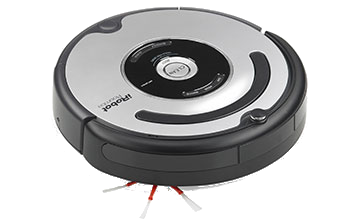
\includegraphics[scale=2.5]{./Figures/roomba.png}
    \caption{iRobot Roomba 500, utilizado como base móvil para este trabajo.\protect\footnotemark}
    \label{fig:roomba}
\end{figure}

\footnotetext{Imagen tomada de \url{https://uncrate.com/assets_c/2009/04/roomba-560-stretched-thumb-960x640-3177.jpg}}

\subsection{Roomba Open Interface}\label{sec:openInterface}
Todos los Roomba lanzados a partir del año 2005 son compatibles con una interfaz de comunicación serial denominada Roomba Open Interface, a la que es posible acceder mediante la conexión a un puerto físico disponible en la placa madre del robot. Esto habilita al usuario a todo tipo de interacción con el hardware del robot, como consultar la lectura de cada uno de sus sensores o comandar sus actuadores. Este protocolo ha sido actualizado a la par de las sucesivas actualizaciones del Roomba para ofrecer nuevas funcionalidades o mejoras y en cada caso, se encuentra acompañado de un documento oficial por parte de iRobot en formato PDF\protect\footnotemark.

\footnotetext{Imagen tomada de \url{https://cdn-shop.adafruit.com/datasheets/create_2_Open_Interface_Spec.pdf}}


\subsection{Conexionado del robot por puerto serie}

En la figura \ref{fig:roombaPinout} y la tabla \ref{tab:Pines} se exponen respectivamente, la distribución de pines en el conector y su conexión correspondiente para entablar comunicación con el robot mediante el puerto Mini-DIN.

\begin{figure}[ht]
    \centering
    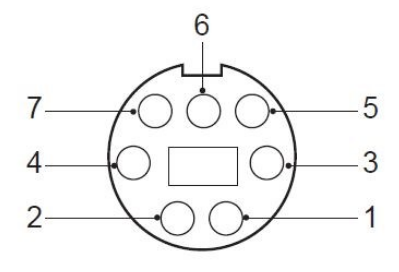
\includegraphics[scale=.4]{./Figures/pinout.png}
    \caption{Distribución de pines en el conector hembra Mini-DIN.}
    \label{fig:roombaPinout}
\end{figure}

\begin{table}[h]
    \centering
    \caption{Referencia de pines en conector Mini-DIN hembra.}
    \label{tab:Pines}
    \begin{tabular}{rll}
        \toprule
        \multicolumn{1}{l}{Pin} & Nombre & Descripción                                  \\
        \midrule
        1                       & Vpwr   & Positivo directo de la batería (no regulado) \\
        2                       & Vpwr   & Positivo directo de la batería (no regulado) \\
        3                       & RXD    & 0 - 5 VCC Entrada serie                      \\
        4                       & TXD    & 0 - 5 VCC Salida serie                       \\
        5                       & BRC    & Cambio de \textit{baud-rate}                 \\
        6                       & GND    & Tierra del robot                             \\
        7                       & GND    & Tierra del robot                             \\
        \bottomrule
    \end{tabular}
\end{table}

\section{Placa de desarrollo STM32-NUCLEO}

Es una familia de placas de desarrollo elaboradas por la compañía ST. Entre sus características principales se destacan:

\begin{itemize}
    \item Bajo costo
    \item Compatibilidad con \textit{shields} de Arduino
    \item Programador/debugger ST-Link integrado
    \item biblioteca del tipo HAL con variados ejemplos de código
\end{itemize}

Con el fin de garantizar la escalabilidad del sistema, para este proyecto se optó por una de las placas mas avanzadas de esta familia, denominada NUCLEO-F746ZG y mostrada en la figura \ref{fig:stm32nucleo}. Esta provee un microcontrolador ARM Cortex-M7 con FPU de doble precisión, 320 kB de RAM, así como 1 MB de Flash. Ofrece además conexión Ethernet y una amplia cantidad de GPIOs.

\begin{figure}[ht]
    \centering
    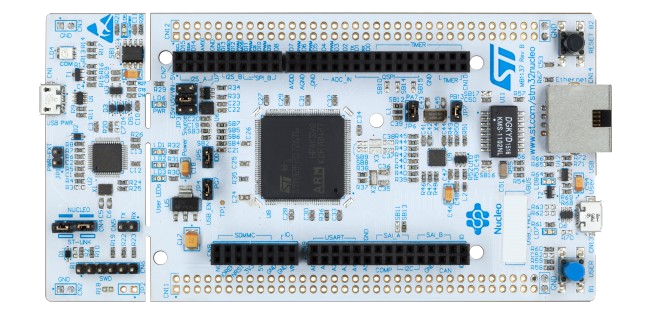
\includegraphics[scale=1.5]{./Figures/stm32nucleo.png}
    \caption{Placa de desarrollo STM32 NUCLEO-F746ZG elegida para comandar el robot.\protect\footnotemark}
    \label{fig:stm32nucleo}
\end{figure}

\footnotetext{Imagen tomada de \url{https://www.carminenoviello.com/wp-content/uploads/2015/12/nucleo_144_large-2-660x330.jpg}}

\section{Sensor Kinect 360}

El Kinect para Xbox 360 o simplemente Kinect, es un dispositivo de captura de movimiento diseñado por la empresa Microsoft que utiliza tecnología desarrollada por la empresa israelita PrimeSense.

Cuenta con una cámara que captura imágenes en formato RGB, un \textit{array} de micrófonos, así como un sensor de profundidad. Si bien existen otras características extra que podrían mencionarse, vale la pena detenerse en esta última y explicar en qué consiste, puesto que se la utilizó de manera extensiva en el trabajo propuesto para la generación de mapas del robot.

\subsection{Imagen de profundidad}

El sensor de profundidad del Kinect consiste en un proyector de nube de puntos infrarrojos combinado con un sensor CMOS monocromático, similar al de una cámara fotográfica. Funcionando en combinación, estos dos elementos son capaces de captar la información necesaria para que un ASIC genere con ella una imagen de profundidad o \textit{Depth map}, que consiste en un mapa de bits con información sobre la distancia relativa entre el sensor y los objetos detectados. En la figura \ref{fig:depthMap} se puede apreciar una imagen de profundidad generada mediante el sensor Kinect en el que se distingue claramente la silueta de una persona en un entorno con diferentes objetos. Las distintas tonalidades de grises visualizadas son una representación de la distancia del objeto al sensor, por lo que para objetos cercanos veremos píxeles de color gris mas claro mientras que para objetos lejanos se verán mas oscuros.

\begin{figure}[ht]
    \centering
    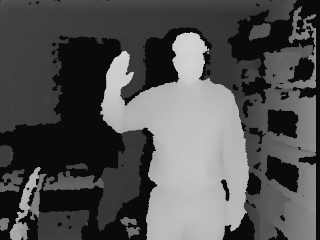
\includegraphics[scale=2.0]{./Figures/depth_map.png}
    \caption{\textit{Depth map} de la silueta de una persona.}
    \label{fig:depthMap}
\end{figure}

\section{Unidad de medición inercial}

Una unidad de medición inercial o IMU por sus siglas en inglés, es un dispositivo electrónico capaz de medir y reportar la velocidad angular y en algunos casos, el campo magnético que rodea al cuerpo.

Las IMU funcionan detectando la aceleración lineal mediante uno o más acelerómetros y la tasa de rotación usando uno o más giroscopios. Algunos de estos dispositivos incluyen también un magnetómetro que se utiliza comúnmente como una referencia de rumbo.

Las configuraciones típicas de una IMU continenen un acelerómetro, un giroscopio y un magnetómetro para cada uno de los tres ejes de giros y fuerzas del vehículo: cabeceo, alabeo y guiñada, que se muestran en la figura ref{fig:imu}. Para el caso particular del robot móvil propuesto en este trabajo, solo se hace uso de las aceleraciones: angular en el eje Z y lineal en el eje X, respectivamente.

\begin{figure}[ht]
    \centering
    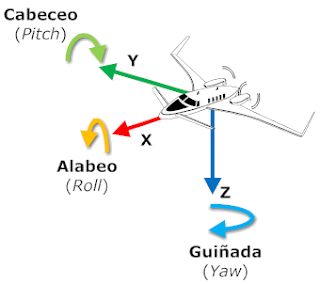
\includegraphics[scale=1.5]{./Figures/imu.png}
    \caption{Ejes de giros y fuerzas de un vehículo.\protect\footnotemark}
    \label{fig:depthMap}
\end{figure}

\footnotetext{Imagen tomada de \url{http://skiras.blogspot.com/2012/10/4copter-conceptos-i-ejes-giros-y-fuerzas.html}}

\subsection{Sensor MPU6050}\label{sec:mpu6050}

El dispositivo MPU-6050 mostrado en la figura \ref{fig:mpu6050} combina en el mismo chip un giroscopio de 3 ejes con un acelerómetro también de 3 ejes. Mediante lo que el fabricante denomina \textit{Digital Motion Processor} o DMP, esta IMU es capaz de procesar algoritmos de fusión de datos de 6 ejes, usualmente ejecutados en un microcontrolador o DSP mediante un filtro de Kalman o similar. Si bien el chip no incluye un magnetómetro, sí ofrece una interfaz I2C que posibilita conectarla a un magnetómetro externo, de este modo el DMP puede aprovechar la información de campo magnético en en sus algoritmos de fusión para generar resultados más precisos.

\begin{figure}[ht]
    \centering
    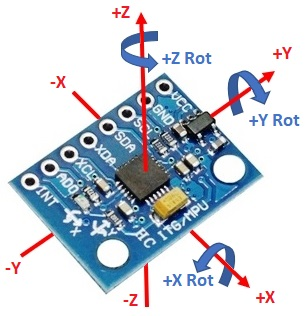
\includegraphics[scale=0.45]{./Figures/mpu6050.jpg}
    \caption{Sensor MPU-6050 con sus ejes de giros y fuerzas.}
    \label{fig:mpu6050}
\end{figure}